\documentclass{article}

% Creative AI Track, single-blind submission.
% Do not add "final" until the paper is accepted.
\usepackage[creativeai]{neurips_2026}

\usepackage[utf8]{inputenc}
\usepackage[T1]{fontenc}
\usepackage{hyperref}
\usepackage{url}
\usepackage{booktabs}
\usepackage{amsfonts}
\usepackage{amsmath}
\usepackage{amssymb}
\usepackage{nicefrac}
\usepackage{microtype}
\usepackage{xcolor}
\usepackage{graphicx}
\usepackage{multirow}
\usepackage{enumitem}
\usepackage{tikz}
\usetikzlibrary{arrows.meta, positioning, shapes.geometric, fit}


\usepackage{longtable}
\usepackage{array}
\usepackage{pdflscape}
\usepackage{ragged2e}
\usepackage{enumitem}
\usepackage[table]{xcolor}
\newcolumntype{L}[1]{>{\RaggedRight\arraybackslash}p{#1}}
\usepackage{float}

\definecolor{intentblue}{RGB}{224,235,252}
\definecolor{referencegreen}{RGB}{225,242,229}
\definecolor{artifactorange}{RGB}{252,235,215}
\definecolor{feedbackpurple}{RGB}{238,228,248}

\title{
Negotiating Creative Agency Through Artifact-Grounded AI Co-Design:
A Joint Aesthetic--Physical Design System for Interactive Fashion
}

% The Creative AI Track uses single-blind review, so author names should be
% included. Replace the placeholders below with the final author information.
\author{
  Lu Sun \\
  Altitut AI \\
  United States \\
  \texttt{lu.sun@altitut.ai}
  \And
  Alfredo Costilla Reyes \\
  Altitut AI / University of California, Davis \\
  United States \\
  \texttt{alfredo@altitut.ai}
  % \And
  % Mengmeng Wang \\
  % Altitut AI \\
  % United States \\
  % \texttt{EMAIL}
}

\begin{document}

\maketitle

some idea: Game platform npc for arts/academic survey/customized own AI buddy/assistant -> video only + paperwork (<=3 pages). FounderCoach for paper/poster (<=6 pages)?

\begin{figure}[H]
    \centering
    
\includegraphics[width=\linewidth]{NeurIPS/NeurIPS_CreativeAI.png}
    \caption{\textit{\textbf{FounderCoach creative co-design pipeline overview.} Artists describe their vision; the system retrieves relevant references, builds a joint aesthetic-physical representation, and generates multiple design alternatives with tradeoffs. Humans select and refine, build prototypes, test in the real world, and feed observations back for revision. All data stays local, works offline, and requires only a one-time hardware cost.}}
    \label{fig:placeholder}
\end{figure}

\begin{landscape}

\begin{longtable}{
    L{0.05\linewidth}
    L{0.08\linewidth}
    L{0.3\linewidth}
    L{0.33\linewidth}
    L{0.15\linewidth}
    L{0.08\linewidth}
}
% \caption{
% Internal execution plan for the NeurIPS 2026 Creative AI submission.
% The plan prioritizes one complete human--AI--artifact iteration, one
% structured design-reference dataset, and one final Gemma comparison before
% the August 3 submission deadline.
% }
% \label{tab:neurips-internal-plan}
% \\

\toprule
\textbf{Dates}
&
\textbf{Workstream}
&
\textbf{Core team responsibilities}
&
\textbf{New intern responsibilities}
&
\textbf{Required outputs}
&
\textbf{Decision gate}
\\
\midrule
\endfirsthead

\multicolumn{6}{l}{
\textit{Table~\ref{tab:neurips-internal-plan} continued from previous page}
}
\\
\toprule
\textbf{Dates}
&
\textbf{Workstream}
&
\textbf{Core team responsibilities}
&
\textbf{New intern responsibilities}
&
\textbf{Required outputs}
&
\textbf{Decision gate}
\\
\midrule
\endhead

\midrule
\multicolumn{6}{r}{\textit{Continued on next page}}
\\
\endfoot

\bottomrule
\endlastfoot

July 8--9
&
\textbf{Scope freeze and creative concept}
&
\begin{itemize}[leftmargin=*,nosep]
    \item Freeze the paper contribution as a
    \textbf{joint aesthetic--physical design representation and
    artifact-grounded agency loop}.
    \item Select one primary artifact:
    a sound-responsive hat or sculptural headpiece.
    \item Define the minimum complete cycle:
    intent $\rightarrow$ references $\rightarrow$ alternatives
    $\rightarrow$ build $\rightarrow$ observation $\rightarrow$ revision.
    \item Confirm that the paper, not a separate artwork submission,
    is the primary deliverable.
\end{itemize}
&
\begin{itemize}[leftmargin=*,nosep]
    \item Review the project brief and existing CircuitCanva /
    FounderCoach prototype.
    \item Create a one-page inventory of available hardware,
    software, fabrication skills, and missing materials.
    \item Identify which parts of the previous IoT Smart Camera
    project can be reused.
\end{itemize}
&
\begin{itemize}[leftmargin=*,nosep]
    \item Frozen research questions.
    \item One selected artifact.
    \item Defined roles and shared folder structure.
    \item Final system name and terminology.
\end{itemize}
&
No expansion to multiple artifacts or multiple creative domains.
\\

\rowcolor{gray!8}
July 9--11
&
\textbf{Reference corpus and semantic search}
&
\begin{itemize}[leftmargin=*,nosep]
    \item Define the creative-reference schema:
    artistic intent, material, component, behavior, power,
    placement, fabrication, source, license, and uncertainty.
    \item Implement the first semantic-search pipeline.
    \item Use Qualcomm and Microchip materials as examples of
    structured technical documentation and design references.
    \item Use Adafruit wearable and fashion projects as
    creative-fabrication precedents.
\end{itemize}
&
\begin{itemize}[leftmargin=*,nosep]
    \item Collect and catalog 30--50 legally usable references:
    wearable projects, component datasheets, tutorials,
    material references, and internally created templates.
    \item Record URL, creator, license or usage status,
    component list, interaction behavior, and fabrication method.
    \item Test 15--20 semantic-search queries and manually label
    relevant and irrelevant retrieval results.
    \item Flag restricted or unclear manufacturer content;
    do not copy restricted source files into the dataset.
\end{itemize}
&
\begin{itemize}[leftmargin=*,nosep]
    \item Structured reference corpus.
    \item Search-query benchmark.
    \item Source and license log.
    \item Initial Recall@K / relevance results.
\end{itemize}
&
Semantic search must return usable creative and technical references
for at least three representative prompts.
\\

July 10--13
&
\textbf{Manual FounderCoach Design Reference}
&
\begin{itemize}[leftmargin=*,nosep]
    \item Define the manually authored gold-standard
    \textbf{FounderCoach Design Reference}.
    \item Recycle the IoT Smart Camera architecture where useful:
    compute module, camera, screen, microphone, power, and software.
    \item Adapt those modules into the selected interactive-fashion
    artifact.
    \item Specify what the AI should generate versus what requires
    human engineering approval.
\end{itemize}
&
\begin{itemize}[leftmargin=*,nosep]
    \item Manually document the complete process:
    requirements, block diagram, component selection, wiring or
    schematic, physical layout, software logic, assembly, and test plan.
    \item Create one Raspberry Pi or microcontroller-based reference
    using camera, screen, microphone, LEDs, and power modules where
    relevant.
    \item Record design rationales and component substitutions.
    \item Photograph each design and assembly stage.
\end{itemize}
&
\begin{itemize}[leftmargin=*,nosep]
    \item Gold-standard design-reference record.
    \item Architecture diagram.
    \item BOM and layout.
    \item Software and interaction logic.
    \item Test checklist.
\end{itemize}
&
The manual reference must be complete enough that another team member
could reproduce the artifact.
\\

\rowcolor{gray!8}
July 11--14
&
\textbf{Manufacturing and fabrication feasibility}
&
\begin{itemize}[leftmargin=*,nosep]
    \item Decide which parts will be built internally and which could
    be externally fabricated.
    \item Treat Shanghai manufacturing as a feasibility and cost
    comparison, not as a deadline-critical dependency.
    \item Define reusable template fields for manufacturing handoff.
\end{itemize}
&
\begin{itemize}[leftmargin=*,nosep]
    \item Prepare a simplified manufacturing package:
    BOM, dimensions, assembly notes, photos, material requirements,
    and expected quantity.
    \item Contact one or two appropriate Shanghai-based fabrication
    or assembly vendors for rough cost, lead-time, minimum-order,
    and manufacturability feedback.
    \item Convert vendor questions and feedback into reusable
    FounderCoach manufacturing-template fields.
\end{itemize}
&
\begin{itemize}[leftmargin=*,nosep]
    \item Manufacturability checklist.
    \item Rough cost and lead-time comparison.
    \item Manufacturing-handoff template.
    \item Risks that must remain human-reviewed.
\end{itemize}
&
External manufacturing must not block the artifact build or paper.
\\

July 12--16
&
\textbf{FounderCoach co-design prototype}
&
\begin{itemize}[leftmargin=*,nosep]
    \item Connect semantic search to the existing FounderCoach /
    CircuitCanva workflow.
    \item Generate a joint representation of:
    aesthetic goal, components, material, placement, software,
    power, fabrication, provenance, and uncertainty.
    \item Add explicit agency controls:
    accept, modify, combine, reject, pin reference, and mark
    constraints as fixed or negotiable.
\end{itemize}
&
\begin{itemize}[leftmargin=*,nosep]
    \item Enter the manual gold-standard reference into the structured
    template.
    \item Run at least five creative prompts through the prototype.
    \item Log missing fields, incorrect components, unsupported claims,
    confusing interface behavior, and failure cases.
    \item Verify that generated references and design claims link back
    to their sources.
\end{itemize}
&
\begin{itemize}[leftmargin=*,nosep]
    \item Functional minimum co-design workflow.
    \item Five documented prompt sessions.
    \item Agency interaction log.
    \item Error and missing-feature list.
\end{itemize}
&
The prototype must support one full prompt-to-build workflow;
polished UI is optional.
\\

\rowcolor{gray!8}
July 14--18
&
\textbf{Base and retrieval experiments}
&
\begin{itemize}[leftmargin=*,nosep]
    \item Freeze a common evaluation set of creative prompts.
    \item Run two initial conditions:
    Base Gemma and retrieval-grounded Gemma.
    \item Define evaluation criteria:
    intent alignment, diversity, feasibility, provenance,
    agency, and manual correction effort.
\end{itemize}
&
\begin{itemize}[leftmargin=*,nosep]
    \item Run identical prompts under both model conditions.
    \item Remove model-condition labels and prepare blinded output sets.
    \item Record component errors, unsupported claims,
    missing constraints, source coverage, and time required for
    manual correction.
    \item Organize output images and text for the paper figures.
\end{itemize}
&
\begin{itemize}[leftmargin=*,nosep]
    \item Base versus RAG comparison.
    \item Qualitative examples.
    \item Preliminary metric table.
    \item Failure-case appendix.
\end{itemize}
&
Continue only with metrics that can be evaluated consistently
before the deadline.
\\

July 16--20
&
\textbf{One final Gemma adaptation experiment}
&
\begin{itemize}[leftmargin=*,nosep]
    \item Prepare one small, structured adaptation dataset using:
    creative intent, references, constraints, alternatives,
    artist choices, design rationale, and test feedback.
    \item Run one lightweight Gemma LoRA or equivalent adaptation.
    \item Keep retrieval active so the experiment tests
    adaptation plus evidence grounding, not memorization.
\end{itemize}
&
\begin{itemize}[leftmargin=*,nosep]
    \item Clean and format the design-reference examples.
    \item Check that train and evaluation prompts do not overlap.
    \item Document dataset size, fields, filtering decisions,
    and removed examples.
    \item Run the frozen prompt set and archive all outputs.
\end{itemize}
&
\begin{itemize}[leftmargin=*,nosep]
    \item Base Gemma results.
    \item RAG Gemma results.
    \item Adapted RAG Gemma results.
    \item One ablation or failure analysis.
\end{itemize}
&
Stop after one defensible experiment.
Do not spend the remaining schedule repeatedly tuning the model.
\\

\rowcolor{gray!8}
July 17--22
&
\textbf{Build and physical testing}
&
\begin{itemize}[leftmargin=*,nosep]
    \item Select one generated alternative with the artist or internal
    creative lead.
    \item Record why it was accepted, modified, combined, or rejected.
    \item Approve low-voltage hardware and wearable-safety decisions.
\end{itemize}
&
\begin{itemize}[leftmargin=*,nosep]
    \item Build the interactive hat or headpiece from the approved
    reference.
    \item Implement microphone-to-light or sensor-to-behavior software.
    \item Test battery runtime, weight, balance, heat,
    response latency, light or sound behavior, and comfort.
    \item Maintain a build diary with photos, failures, fixes,
    time, and cost.
\end{itemize}
&
\begin{itemize}[leftmargin=*,nosep]
    \item One functional physical artifact.
    \item Test measurements.
    \item Build diary.
    \item Before-and-after design comparison.
\end{itemize}
&
A visually and behaviorally demonstrable artifact is required;
a perfect enclosure is not.
\\

July 21--24
&
\textbf{Agency and revision study}
&
\begin{itemize}[leftmargin=*,nosep]
    \item Conduct one complete artifact-grounded revision cycle.
    \item Ask where the AI enabled, steered, constrained, or failed
    the creative process.
    \item Capture examples of refusal, modification, hidden assumptions,
    and material resistance.
\end{itemize}
&
\begin{itemize}[leftmargin=*,nosep]
    \item Prepare interview or reflection prompts.
    \item Record artist decisions at each stage.
    \item Enter physical observations into FounderCoach.
    \item Generate and document the revised design.
    \item Code feedback into themes:
    ownership, control, steering, refusal, usefulness, and friction.
\end{itemize}
&
\begin{itemize}[leftmargin=*,nosep]
    \item Complete human--AI--artifact loop.
    \item Agency case-study evidence.
    \item Revised output.
    \item Quotable but consented reflections.
\end{itemize}
&
The paper must show agency through observed decisions,
not only through conceptual discussion.
\\

\rowcolor{gray!8}
July 22--26
&
\textbf{Paper draft and figures}
&
\begin{itemize}[leftmargin=*,nosep]
    \item Draft Introduction, Related Work, System,
    Agency Analysis, Study, Results, Limitations, and Conclusion.
    \item Reduce the contribution to two or three central claims.
    \item Create the final pipeline figure and experiment table.
\end{itemize}
&
\begin{itemize}[leftmargin=*,nosep]
    \item Prepare clean screenshots, artifact photographs,
    architecture diagrams, and captions.
    \item Verify every reported number against the experiment log.
    \item Assemble supplementary build and dataset documentation.
\end{itemize}
&
\begin{itemize}[leftmargin=*,nosep]
    \item Complete first paper draft.
    \item Final system figure.
    \item Model-comparison table.
    \item Artifact progression figure.
\end{itemize}
&
By July 26, no new core feature may be added.
\\

July 25--28
&
\textbf{Results freeze and internal review}
&
\begin{itemize}[leftmargin=*,nosep]
    \item Freeze experimental results.
    \item Review whether claims match evidence.
    \item Remove unsupported claims about creativity,
    generalization, autonomy, or engineering reliability.
    \item Check fit with the Creative AI theme of Agency.
\end{itemize}
&
\begin{itemize}[leftmargin=*,nosep]
    \item Reproduce key outputs from saved prompts and configurations.
    \item Check links, citations, figure labels, and dataset records.
    \item Create a short limitations list from observed failures.
\end{itemize}
&
\begin{itemize}[leftmargin=*,nosep]
    \item Reproducible result package.
    \item Claim--evidence checklist.
    \item Final limitations and ethics notes.
\end{itemize}
&
No new training run unless an existing result is invalid.
\\

\rowcolor{gray!8}
July 27--30
&
\textbf{Video, poster, and supplementary media}
&
\begin{itemize}[leftmargin=*,nosep]
    \item Script a concise visual narrative:
    intent, AI alternatives, artist choice, build,
    physical behavior, failure, and revision.
    \item Prepare poster-compatible figures even though the paper is
    the primary submission.
\end{itemize}
&
\begin{itemize}[leftmargin=*,nosep]
    \item Record clean artifact video and screen capture.
    \item Edit a two-to-three-minute internal preview.
    \item Export high-resolution photos and a thumbnail.
    \item Add captions and source attributions.
\end{itemize}
&
\begin{itemize}[leftmargin=*,nosep]
    \item Demo video.
    \item Thumbnail.
    \item Poster figure set.
    \item Supplementary-media folder.
\end{itemize}
&
Video must demonstrate interaction and iteration,
not only show a finished object.
\\

July 29--31
&
\textbf{Final paper revision}
&
\begin{itemize}[leftmargin=*,nosep]
    \item Compress the paper to the official 2--6 page content limit.
    \item Ensure author names remain included for single-blind review.
    \item Verify references, ethics, safety, agency framing,
    and author contributions.
\end{itemize}
&
\begin{itemize}[leftmargin=*,nosep]
    \item Proofread tables and captions.
    \item Verify that all images are legible in grayscale and color.
    \item Confirm that source files compile using the official template.
\end{itemize}
&
\begin{itemize}[leftmargin=*,nosep]
    \item Submission-ready PDF.
    \item Supplementary files.
    \item Final authorship and contribution record.
\end{itemize}
&
Internal approval by July 31.
\\

\rowcolor{gray!8}
August 1
&
\textbf{Submission rehearsal}
&
\begin{itemize}[leftmargin=*,nosep]
    \item Upload a complete draft to OpenReview.
    \item Check PDF rendering, author information, abstract,
    keywords, conflicts, and supplementary files.
\end{itemize}
&
\begin{itemize}[leftmargin=*,nosep]
    \item Independently inspect the uploaded PDF and media.
    \item Confirm that no files expose private participant information
    or restricted manufacturer content.
\end{itemize}
&
\begin{itemize}[leftmargin=*,nosep]
    \item Validated OpenReview draft.
    \item Submission checklist.
\end{itemize}
&
All required fields and files must be accepted by the portal.
\\

August 2
&
\textbf{Final corrections}
&
\begin{itemize}[leftmargin=*,nosep]
    \item Make only evidence, clarity, citation, and formatting fixes.
    \item Obtain final approval from all authors.
\end{itemize}
&
\begin{itemize}[leftmargin=*,nosep]
    \item Perform final citation, figure, and supplementary-media check.
\end{itemize}
&
Final submission package.
&
No new experiment or feature.
\\

\rowcolor{gray!8}
August 3 AoE
&
\textbf{Submission buffer}
&
Submit before the final hours of the Anywhere-on-Earth deadline.
&
Remain available only for file verification or emergency correction.
&
OpenReview confirmation and archived submission package.
&
Submitted.
\\

\end{longtable}

\end{landscape}

\begin{itemize}
    \item manually construct the gold-standard FounderCoach Design Reference;
    \item document the Raspberry Pi or microcontroller, camera, screen,
    microphone, LED, power, and software integration process;
    \item convert the manual design--build--test process into structured
    reusable templates;
    \item collect and label creative and technical references for semantic search;
    \item build and test the interactive fashion artifact;
    \item document failures, corrections, measurements, cost, and time;
    \item prepare screenshots, photographs, diagrams, and demo video materials;
    \item support the Base Gemma, RAG Gemma, and adapted Gemma comparison by
    formatting inputs and logging outputs.
\end{itemize}





\begin{abstract}
Generative AI can rapidly produce fashion images and visual variations, but image generation alone does not help artists determine how an interactive garment or wearable artwork can be physically built, tested, and revised. We present a proposed artifact-grounded co-creative system that translates multimodal artistic intent into a joint representation of aesthetic goals, electronic components, materials, spatial relationships, fabrication constraints, and physical uncertainty. The system retrieves relevant creative and technical references, generates multiple interpretable design alternatives, supports human selection and refusal, and incorporates evidence from a fabricated artifact into subsequent design iterations. We frame creative agency not as a fixed property of either the artist or the model, but as something negotiated across artist decisions, model suggestions, retrieved precedents, technical constraints, sensors, and physical materials. The initial study centers on an interactive sound-responsive fashion artifact and compares a base Gemma model, retrieval-grounded Gemma, and an adapted Gemma model with structured creative-reference retrieval. We propose mixed-method evaluation of artistic-intent alignment, design diversity, physical feasibility, explanation quality, artist-perceived agency, manual correction effort, and post-fabrication improvement. The contribution is a framework for creative AI that moves beyond visual ideation toward embodied, accountable, and revisable human--AI co-creation.
\end{abstract}

\section{Introduction}

Generative AI has substantially expanded the speed and volume of visual
ideation available to artists and designers. Text-to-image systems can produce
many stylistic variations of a garment, accessory, installation, or speculative
object within seconds. However, visual abundance does not necessarily increase
creative agency. A system may appear to empower an artist while implicitly
steering the artist toward patterns encoded in its training data, interface,
default prompts, or optimization objectives.

The gap becomes especially visible in interactive fashion and wearable art.
A generated image may depict a luminous hat, responsive garment, or kinetic
headpiece, but it does not specify how the work should be physically
constructed. The artist must still reason about materials, weight distribution,
electrical components, sensors, power consumption, thermal behavior, comfort,
fabrication procedures, and safety. The transition from image to artifact
therefore exposes a boundary between apparent creative possibility and
physical agency.

This paper proposes the \textbf{FounderCoach Creative Reference Engine}, an
artifact-grounded human--AI co-design system for interactive fashion and
wearable art. The system accepts multimodal expressions of creative intent,
retrieves relevant artistic and technical references, constructs a joint
aesthetic--physical design representation, and generates multiple physically
differentiated alternatives. The artist may accept, modify, combine, postpone,
or reject the system's recommendations. After fabrication, images, videos,
measurements, and reflective feedback are returned to the system to support a
new design iteration.

The central premise is that creative agency should not be evaluated only at the
moment a prompt is written or an image is generated. Agency is negotiated
throughout a longer process:

\begin{quote}
artistic intention $\rightarrow$ reference interpretation $\rightarrow$
alternative generation $\rightarrow$ human selection $\rightarrow$
fabrication $\rightarrow$ embodied observation $\rightarrow$ revision.
\end{quote}

The proposed work contributes:

\begin{enumerate}[leftmargin=*]
    \item a joint aesthetic--physical representation connecting artistic
    intention to materials, electronics, fabrication, and uncertainty;
    \item a retrieval-grounded co-design workflow that produces alternatives
    with explicit aesthetic and technical tradeoffs;
    \item an artifact-grounded revision loop in which physical evidence changes
    subsequent model recommendations;
    \item an agency-centered evaluation framework spanning artist control,
    model initiative, constraint visibility, refusal, and accountability; and
    \item an empirical comparison of base, retrieval-grounded, and adapted
    Gemma-based systems in an interactive-fashion design task.
\end{enumerate}

\section{Background and related work}

\subsection{Creative AI and co-creative systems}

Creativity-support systems have long sought to extend human ideation without
eliminating human judgment. Prior work distinguishes between tools that support
creative action and systems that participate more actively in a co-creative
process \citep{lubart2005,frich2019}. Human--AI collaboration introduces
questions about initiative, turn-taking, interpretation, control, and
responsibility. A productive co-creative system should not merely maximize
output quantity; it should allow users to understand, redirect, and contest the
system's contribution \citep{amershi2019,shneiderman2020}.

Recent fashion-oriented AI systems have explored visual ideation, style
generation, sketch retrieval, and designer-guided customization. For example,
HAIGEN combines generative models and designer-specific adaptation to support
human--AI fashion ideation \citep{jiang2024haigen}. Such systems demonstrate the
potential of collaborative fashion AI, but the dominant output remains a
visual representation rather than a physically validated artifact.

\subsection{Agency in generative design}

The NeurIPS 2026 Creative AI theme asks how agency is asserted, delegated,
shared, constrained, resisted, or redistributed in creative practice with AI
\citep{neurips2026creative}. In generative design, agency cannot be reduced to
whether a user entered a prompt. Models influence which options appear,
interfaces determine which controls are visible, datasets shape aesthetic
priors, and ranking mechanisms determine which alternatives receive attention.

We therefore treat agency as a process distributed across several actors:

\begin{itemize}[leftmargin=*]
    \item \textbf{the artist}, who defines intention, interprets alternatives,
    refuses suggestions, and authorizes fabrication;
    \item \textbf{the model}, which proposes combinations, identifies
    relationships, and introduces variation;
    \item \textbf{the reference corpus}, which constrains what precedents,
    components, and fabrication methods are made visible;
    \item \textbf{the interface}, which structures available choices and
    explanations;
    \item \textbf{the artifact}, whose material behavior may resist both human
    and model expectations; and
    \item \textbf{the surrounding technical system}, including sensors,
    electrical limits, safety requirements, and fabrication infrastructure.
\end{itemize}

This framing avoids treating agency as a zero-sum transfer between artist and
AI. Instead, it asks where initiative appears, where it is constrained, and who
retains authority to interpret and act.

\subsection{Retrieval-grounded generation and model adaptation}

Retrieval-augmented generation can ground model output in external documents
rather than relying exclusively on parametric memory \citep{lewis2020rag}.
For creative-technical tasks, retrieval can provide fabrication methods,
component specifications, prior artwork, and relevant safety information.
However, retrieval also creates curatorial power: the system influences the
artist by deciding which references are surfaced and how they are framed.

Gemma provides an open family of language models suitable for adaptation and
controlled experimentation \citep{gemma2024}. In this work, Gemma is an
implementation component rather than the primary contribution. The central
research question is whether structured representations, retrieval, and
artifact feedback change the quality and agency dynamics of co-design.

\subsection{Embodied and artifact-grounded iteration}

Physical artifacts introduce forms of evidence that cannot be fully captured
by text or images. Material flexibility, balance, heat, acoustic response,
wearer comfort, and construction difficulty may contradict the design's
predicted behavior. Real-to-sim-to-real research in robotics demonstrates the
value of updating models using evidence from physical systems
\citep{torne2024}. We adapt this principle to creative practice: the artifact is
not merely an output but an active participant that reveals hidden constraints
and motivates reinterpretation.

\section{Research questions}

The proposed study addresses five research questions.

\paragraph{RQ1: Multimodal intent representation.}
Can a system translate ambiguous artistic language, sketches, mood boards, and
reference images into an interpretable combination of aesthetic objectives and
physical constraints?

\paragraph{RQ2: Retrieval-grounded creative adaptation.}
Can structured retrieval improve feasibility and traceability without causing
the system to imitate a single precedent or reduce creative diversity?

\paragraph{RQ3: Aesthetic--physical tradeoff reasoning.}
Can a joint design representation generate alternatives that preserve artistic
intent while making power, material, comfort, weight, and fabrication
tradeoffs visible?

\paragraph{RQ4: Human agency and refusal.}
Can the system exercise useful initiative while preserving the artist's ability
to redirect, defer, reject, or reinterpret its suggestions?

\paragraph{RQ5: Artifact-grounded revision.}
Does evidence from a fabricated artifact improve the technical feasibility and
artistic coherence of subsequent design alternatives?

\section{System overview}

\subsection{Co-design workflow}

Figure~\ref{fig:workflow} illustrates the proposed workflow. The system begins
with a multimodal expression of creative intent. It then retrieves artistic and
technical references, builds a joint design graph, generates multiple
alternatives, supports human selection and modification, and incorporates
artifact feedback into later iterations.

\begin{figure}[t]
\centering
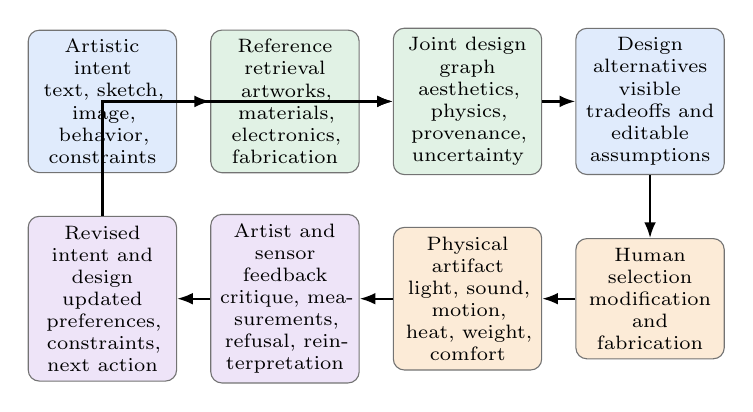
\begin{tikzpicture}[
    node distance=0.42cm,
    every node/.style={
        font=\scriptsize,
        align=center,
        rounded corners,
        minimum height=0.82cm,
        text width=1.65cm,
        draw=black!55
    },
    arrow/.style={-{Latex[length=2mm]}, thick}
]
\node[fill=intentblue] (intent) {
    Artistic intent\\
    text, sketch, image,\\
    behavior, constraints
};

\node[fill=referencegreen, right=of intent] (retrieval) {
    Reference retrieval\\
    artworks, materials,\\
    electronics, fabrication
};

\node[fill=referencegreen, right=of retrieval] (graph) {
    Joint design graph\\
    aesthetics, physics,\\
    provenance, uncertainty
};

\node[fill=intentblue, right=of graph] (alternatives) {
    Design alternatives\\
    visible tradeoffs and\\
    editable assumptions
};

\node[fill=artifactorange, below=0.8cm of alternatives] (fabrication) {
    Human selection\\
    modification and\\
    fabrication
};

\node[fill=artifactorange, left=of fabrication] (artifact) {
    Physical artifact\\
    light, sound, motion,\\
    heat, weight, comfort
};

\node[fill=feedbackpurple, left=of artifact] (feedback) {
    Artist and sensor feedback\\
    critique, measurements,\\
    refusal, reinterpretation
};

\node[fill=feedbackpurple, left=of feedback] (revision) {
    Revised intent and design\\
    updated preferences,\\
    constraints, next action
};

\draw[arrow] (intent) -- (retrieval);
\draw[arrow] (retrieval) -- (graph);
\draw[arrow] (graph) -- (alternatives);
\draw[arrow] (alternatives) -- (fabrication);
\draw[arrow] (fabrication) -- (artifact);
\draw[arrow] (artifact) -- (feedback);
\draw[arrow] (feedback) -- (revision);
\draw[arrow] (revision) |- (graph);

\end{tikzpicture}
\caption{
Proposed artifact-grounded co-design workflow. Agency is negotiated across
artist intention, retrieved precedents, model-generated alternatives,
fabrication decisions, and the physical behavior of the resulting artifact.
}
\label{fig:workflow}
\end{figure}

\subsection{Multimodal creative-intent input}

The system will accept:

\begin{itemize}[leftmargin=*]
    \item natural-language descriptions of mood, narrative, symbolism, and
    intended interaction;
    \item sketches, reference images, and mood boards;
    \item desired light, sound, movement, and sensor behavior;
    \item preferred materials, colors, silhouettes, and fabrication methods;
    \item explicit practical constraints such as budget, weight, battery life,
    comfort, and available skills; and
    \item negative preferences and refusal statements, such as ``avoid a
    polished commercial appearance'' or ``do not hide the wiring.''
\end{itemize}

The explicit inclusion of negative preferences is important for agency. It
allows artists to define boundaries rather than only request additions.

\subsection{Creative-reference retrieval}

A hybrid retrieval system will search a curated corpus containing:

\begin{itemize}[leftmargin=*]
    \item wearable-art precedents and artist-provided references;
    \item openly licensed maker tutorials and fabrication practices;
    \item component datasheets and application notes;
    \item material properties and assembly methods;
    \item internally created design templates; and
    \item prior prompt--design--artifact--revision examples.
\end{itemize}

Retrieval will combine semantic similarity with structured filters such as
component type, interaction modality, fabrication difficulty, weight, power,
and material category. Each retrieved item will retain source provenance and
usage-right metadata.

The system will expose retrieved references to the artist rather than hiding
them behind model output. This enables the artist to inspect, remove, or replace
the precedents influencing the generation.

\subsection{Joint aesthetic--physical design representation}

The core representation will be a heterogeneous design graph

\begin{equation}
G = (V, E),
\end{equation}

where nodes $V$ represent artistic intentions, sensory behaviors, materials,
components, spatial regions, fabrication operations, constraints, evidence,
and observations. Edges $E$ represent relationships such as:

\begin{itemize}[leftmargin=*]
    \item \emph{expresses}: a lighting behavior expresses an artistic intention;
    \item \emph{requires}: a behavior requires a sensor or computation module;
    \item \emph{mounted-on}: an electronic component occupies a physical
    region;
    \item \emph{constrains}: weight, heat, or flexibility limits a design
    choice;
    \item \emph{derived-from}: a recommendation is linked to a reference;
    \item \emph{conflicts-with}: two aesthetic or technical objectives are in
    tension; and
    \item \emph{observed-in}: a physical outcome is associated with a fabricated
    artifact.
\end{itemize}

Each design claim $c_i$ will be associated with provenance $p_i$, verification
status $v_i$, and confidence or uncertainty $u_i$:

\begin{equation}
c_i = (p_i, v_i, u_i).
\end{equation}

The representation is intended to make tradeoffs visible. For example, an
increase in LED density may support a desired visual effect while increasing
power demand, heat, wiring complexity, and stiffness.

\subsection{Alternative generation}

Instead of producing one ``best'' design, the system will generate a set of
alternatives:

\begin{equation}
\mathcal{D} = \{D_1, D_2, \dots, D_k\},
\end{equation}

where each $D_j$ contains:

\begin{itemize}[leftmargin=*]
    \item an aesthetic interpretation;
    \item interaction behavior;
    \item material and component choices;
    \item spatial placement;
    \item estimated power, weight, heat, and fabrication difficulty;
    \item supporting references;
    \item unresolved assumptions; and
    \item suggested next actions.
\end{itemize}

The alternatives will be deliberately differentiated. One may prioritize
visual expressiveness, another comfort, another transparency of construction,
and another ease of fabrication. The system will not automatically rank one
alternative as universally superior.

\subsection{Agency controls}

The interface will include explicit mechanisms for negotiating agency:

\begin{itemize}[leftmargin=*]
    \item \textbf{initiative control}: the artist may choose whether the system
    proposes, critiques, asks questions, or waits;
    \item \textbf{reference control}: the artist may inspect, remove, pin, or add
    retrieved precedents;
    \item \textbf{constraint control}: the artist may mark constraints as fixed,
    negotiable, or intentionally unresolved;
    \item \textbf{refusal}: the artist may reject a suggestion without requiring
    a replacement;
    \item \textbf{traceability}: recommendations display the references and
    assumptions that influenced them;
    \item \textbf{versioning}: discarded designs remain visible as part of the
    creative history; and
    \item \textbf{human authorization}: fabrication-relevant changes require
    explicit human confirmation.
\end{itemize}

These controls are not treated only as usability features. They operationalize
the paper's account of agency.

\section{Creative artifact}

\subsection{Interactive fashion case study}

The initial artifact will be a sound-responsive hat or sculptural headpiece
integrating:

\begin{itemize}[leftmargin=*]
    \item a microphone or sound-level sensor;
    \item a microcontroller;
    \item addressable LEDs;
    \item a rechargeable battery;
    \item textile or lightweight structural material; and
    \item optional motion, proximity, or environmental sensing.
\end{itemize}

Wearable-electronics maker communities demonstrate practical combinations of
lighting, sound response, microcontrollers, wireless control, and expressive
physical form \citep{adafruitwearables}. These examples provide useful
precedents, but they are generally fixed project instructions rather than
adaptive co-design systems.

\subsection{Example creative prompt}

An example prompt is:

\begin{quote}
``Create a lightweight headpiece whose lighting reacts to my voice and becomes
increasingly fragmented as the surrounding soundscape becomes more chaotic. The
work should feel handmade and slightly unstable rather than polished or
commercial.''
\end{quote}

The system may translate this prompt into:

\begin{itemize}[leftmargin=*]
    \item a relationship between voice amplitude, environmental sound
    variability, and light fragmentation;
    \item material options that preserve visible construction;
    \item several LED diffusion and placement strategies;
    \item alternative mappings from sound to color, rhythm, and interruption;
    \item component placement options balancing weight and visibility; and
    \item unresolved artistic questions, such as whether instability should be
    represented through flicker, asymmetry, delay, or incomplete response.
\end{itemize}

\subsection{Role of the physical artifact}

The fabricated object is not treated as a passive realization of the model's
proposal. It may resist the design through:

\begin{itemize}[leftmargin=*]
    \item unexpected weight or imbalance;
    \item excessive wiring stiffness;
    \item uncomfortable heat;
    \item poor light diffusion;
    \item sensor behavior that fails in noisy environments;
    \item an interaction that feels too predictable; or
    \item an aesthetic outcome that is technically correct but artistically
    unsatisfying.
\end{itemize}

These failures are treated as creative evidence. The artist may decide that a
technical imperfection should be preserved, exaggerated, or incorporated into
the work rather than eliminated.

\section{Model conditions and implementation}

\subsection{Condition A: Base Gemma}

The first condition will use a base Gemma model without project-specific
retrieval or adaptation. It will receive the same artist prompt and general
task instructions as the other conditions.

This condition represents a conventional generative-assistant baseline.

\subsection{Condition B: Retrieval-grounded Gemma}

The second condition will augment Gemma with retrieved creative references,
component documentation, material information, and fabrication guidance.

The model will be required to:

\begin{itemize}[leftmargin=*]
    \item cite retrieved evidence for technical claims;
    \item separate sourced information from inferred suggestions;
    \item expose unresolved assumptions; and
    \item generate multiple alternatives rather than one answer.
\end{itemize}

\subsection{Condition C: Adapted Gemma with structured retrieval}

The third condition will use lightweight adaptation, such as LoRA, on a small
structured corpus containing:

\begin{itemize}[leftmargin=*]
    \item creative intentions;
    \item retrieved references;
    \item aesthetic and physical constraints;
    \item generated alternatives;
    \item artist selections and refusals;
    \item prototype observations;
    \item revision rationales; and
    \item final design decisions.
\end{itemize}

The adapted model will retain retrieval access. The purpose of adaptation is not
to train a general fashion model, but to test whether structured co-design
examples improve the model's ability to negotiate aesthetic--physical tradeoffs
and preserve artist-defined constraints.

\subsection{System ablations}

Where time permits, the study will include the following ablations:

\begin{enumerate}[leftmargin=*]
    \item no retrieval;
    \item retrieval without source visibility;
    \item retrieval with source visibility but no structured design graph;
    \item retrieval with the joint aesthetic--physical graph;
    \item full system with artifact feedback.
\end{enumerate}

These comparisons will help determine whether improvements come from model
adaptation, retrieved information, explicit representation, or physical
feedback.

\section{Study design}

\subsection{Participants}

The initial exploratory study will recruit approximately 6--12 participants,
depending on available time and ethics approval. Participants may include:

\begin{itemize}[leftmargin=*]
    \item fashion or visual designers;
    \item artists working with physical media;
    \item makers or wearable-electronics practitioners; and
    \item participants with creative interests but limited electronics
    experience.
\end{itemize}

The study will report participants' relevant experience rather than assume a
single definition of ``artist'' or ``expert.''

If the submission deadline does not permit a completed participant study, the
initial paper will report an expert case study and clearly label the broader
user evaluation as planned work.

\subsection{Tasks}

Each participant will:

\begin{enumerate}[leftmargin=*]
    \item describe an intended interactive-fashion concept;
    \item review outputs from one or more system conditions;
    \item inspect and modify retrieved references and constraints;
    \item select, combine, or reject generated alternatives;
    \item explain important design decisions;
    \item review the feasibility implications of the selected design; and
    \item evaluate revised alternatives following simulated or physical
    artifact feedback.
\end{enumerate}

At least one complete design will proceed through physical fabrication.

\subsection{Artifact-grounded iteration}

The complete case-study cycle will be:

\begin{equation}
\begin{aligned}
\text{Intent}
&\rightarrow \text{Alternatives}
\rightarrow \text{Artist selection} \\
&\rightarrow \text{Fabrication}
\rightarrow \text{Observation}
\rightarrow \text{Critique}
\rightarrow \text{Revision}.
\end{aligned}
\end{equation}

Physical evidence may include:

\begin{itemize}[leftmargin=*]
    \item battery runtime;
    \item component and surface temperature;
    \item total weight;
    \item sound-response latency;
    \item light-response behavior;
    \item photos and video;
    \item construction difficulty; and
    \item artist reflection.
\end{itemize}

\section{Evaluation}

\subsection{Creative outcomes}

Creative evaluation will consider:

\begin{itemize}[leftmargin=*]
    \item alignment with the artist's stated intention;
    \item novelty relative to retrieved references;
    \item diversity across alternatives;
    \item perceived coherence of visual and interactive behavior;
    \item support for exploration rather than premature convergence; and
    \item whether unexpected outputs were useful, distracting, or coercive.
\end{itemize}

Novelty will not be treated as automatically positive. Participants will be
asked whether variation expanded their creative possibilities or merely
increased the number of options.

\subsection{Physical and technical outcomes}

Technical evaluation will consider:

\begin{itemize}[leftmargin=*]
    \item component compatibility;
    \item power and interface consistency;
    \item physical feasibility;
    \item fabrication completeness;
    \item unsupported or incorrect technical claims;
    \item number of expert corrections;
    \item prototype success;
    \item post-fabrication revision quality; and
    \item traceability of safety-relevant recommendations.
\end{itemize}

\subsection{Agency outcomes}

Agency evaluation will examine:

\begin{itemize}[leftmargin=*]
    \item perceived ownership of the final design;
    \item ability to redirect the system;
    \item ability to refuse suggestions;
    \item visibility of model assumptions and references;
    \item perceived model overreach;
    \item whether the system enabled or steered creative decisions;
    \item where participants attributed authorship;
    \item whether constraints felt supportive or restrictive; and
    \item whether fabrication changed the distribution of agency.
\end{itemize}

We will use short Likert-scale questions, semi-structured interviews, and
interaction logs. Example interview questions include:

\begin{quote}
``At what point did the system feel most helpful?''

``At what point did it feel as if the system was deciding for you?''

``Which suggestions did you reject, and why?''

``Did the physical artifact confirm or challenge your original intention?''

``Who or what do you consider responsible for the final form of the work?''
\end{quote}

\subsection{Planned quantitative comparison}

Table~\ref{tab:planned} summarizes the planned comparison.

\begin{table}[t]
\caption{
Planned comparison across model conditions. The central test is whether
retrieval, explicit representation, and artifact feedback improve feasibility
without reducing artist-perceived agency or creative diversity.
}
\label{tab:planned}
\centering
\small
\begin{tabular}{p{0.27\linewidth}ccc}
\toprule
Metric &
Base Gemma &
RAG Gemma &
Adapted RAG Gemma \\
\midrule
Intent alignment & TBD & TBD & TBD \\
Alternative diversity & TBD & TBD & TBD \\
Physical feasibility & TBD & TBD & TBD \\
Source traceability & TBD & TBD & TBD \\
Manual corrections & TBD & TBD & TBD \\
Artist-perceived agency & TBD & TBD & TBD \\
Post-artifact improvement & N/A & TBD & TBD \\
\bottomrule
\end{tabular}
\end{table}

Because this is currently a draft, no numerical results are claimed. The final
submission will distinguish completed results from proposed future work.

\section{Agency analysis}

\subsection{Artist agency}

The artist retains authority over:

\begin{itemize}[leftmargin=*]
    \item interpretation of the creative prompt;
    \item selection or rejection of references;
    \item definition of non-negotiable constraints;
    \item acceptance, modification, or refusal of suggestions;
    \item authorization of fabrication; and
    \item interpretation of failure.
\end{itemize}

The system is designed to preserve disagreement. A rejected suggestion remains
part of the visible process rather than disappearing as an error.

\subsection{Model agency}

The model exercises bounded initiative by:

\begin{itemize}[leftmargin=*]
    \item proposing alternative interpretations;
    \item identifying hidden physical dependencies;
    \item surfacing conflicts;
    \item suggesting references and fabrication strategies; and
    \item asking clarifying questions.
\end{itemize}

However, model initiative is constrained by evidence requirements, explicit
artist controls, and human authorization for fabrication-relevant decisions.

\subsection{Agency of references and datasets}

Retrieved references influence which possibilities appear plausible. A corpus
dominated by commercially polished wearables may suppress handmade,
experimental, disabled, culturally specific, or low-resource forms of creative
practice.

The system will therefore expose reference sources and permit artists to remove,
replace, or expand them. Corpus composition will be reported as part of the
creative method, not treated as neutral infrastructure.

\subsection{Agency of materials and artifacts}

Physical materials introduce resistance, unpredictability, and temporal delay.
These qualities can preserve creative agency by interrupting the speed and
abundance favored by generative systems.

A material failure may produce an artistically meaningful outcome that neither
the artist nor model anticipated. The system should therefore allow the artist
to mark a ``failure'' as a desired feature rather than automatically optimizing
it away.

\subsection{Accountability}

Responsibility remains differentiated:

\begin{itemize}[leftmargin=*]
    \item the model may propose;
    \item the system may warn;
    \item the artist may interpret;
    \item a technical reviewer may verify;
    \item and the fabricator authorizes construction.
\end{itemize}

The system will not claim that model-generated electrical or safety guidance
eliminates the need for qualified human review.

\section{Ethics, safety, and intellectual property}

\subsection{Electrical and wearable safety}

Interactive wearables place electronics close to the human body. Relevant risks
include battery damage, overheating, exposed conductors, excessive weight,
sharp structures, and unsafe charging.

The prototype will use low-voltage components, protected batteries, insulated
connections, conservative power limits, and human technical review. The system
will explicitly distinguish artistic suggestions from safety-critical
engineering claims.

\subsection{Reference provenance and creative appropriation}

Retrieval-grounded creative systems may unintentionally imitate artists or
reuse culturally significant forms without context. Each retrieved creative
reference will retain source attribution where available. The system will avoid
presenting direct stylistic imitation as an unproblematic design strategy.

Participants will be able to exclude specific artists, sources, or aesthetic
traditions from retrieval.

\subsection{Data and participant privacy}

Participant sketches, reflections, preferences, and prototype recordings will
be collected only with consent. The system will distinguish between data used
for the current session, data retained for research analysis, and data approved
for model adaptation.

\subsection{Authorship and disclosure}

The final work will document:

\begin{itemize}[leftmargin=*]
    \item the artist's contributions;
    \item model-generated content;
    \item retrieved references;
    \item engineering and fabrication contributions;
    \item human edits and refusals; and
    \item the role of artifact feedback.
\end{itemize}

This process-based disclosure is more informative than assigning a single
percentage of authorship to the AI.

\section{Limitations}

The proposed study has several limitations.

First, a small participant sample cannot support broad claims about all artists
or designers. The initial work should be interpreted as an exploratory system
and artifact study.

Second, interactive fashion represents only one creative domain. The joint
aesthetic--physical representation may require substantial modification for
architecture, choreography, sculpture, or performance.

Third, a curated corpus may encode selection bias. Source visibility does not
eliminate this bias, although it makes it more inspectable.

Fourth, model explanations may appear more authoritative than their evidence
supports. Provenance and uncertainty indicators reduce but do not eliminate
this risk.

Fifth, successful construction of one artifact does not establish general
engineering reliability. The system remains a co-design and reasoning aid, not
an autonomous engineering authority.

Finally, evaluation of creativity and agency is interpretive. Quantitative
ratings will therefore be combined with interviews, design histories, rejected
alternatives, and artifact documentation.

\section{Discussion}

\subsection{From abundance to accountable alternatives}

Generative systems commonly frame creativity as the production of abundant
variation. Our approach instead emphasizes accountable alternatives:
suggestions whose origins, constraints, and consequences can be inspected.

The goal is not to slow creativity for its own sake, but to create moments in
which the artist can understand what the system is doing and decide whether to
continue.

\subsection{Friction as a creative resource}

Fabrication introduces friction, delay, and failure. In conventional automation,
these may be treated as inefficiencies. In creative practice, they may preserve
judgment and produce reflection.

A system focused only on efficiency might automatically resolve conflicting
constraints. An agency-centered system may instead present the conflict to the
artist and allow it to remain unresolved.

\subsection{Does feasibility constrain creativity?}

Physical feasibility can support agency by helping artists realize ideas that
would otherwise remain images. It can also narrow possibilities if the system
prematurely rejects unconventional designs.

FounderCoach will therefore distinguish:

\begin{itemize}[leftmargin=*]
    \item impossible under known physical constraints;
    \item unsupported by available evidence;
    \item possible but high-risk;
    \item possible with modification; and
    \item intentionally unresolved.
\end{itemize}

This vocabulary creates space for speculation without disguising uncertainty.

\subsection{Beyond interactive fashion}

The same framework could support other creative practices in which aesthetic
intent interacts with physical systems, including:

\begin{itemize}[leftmargin=*]
    \item interactive sculpture;
    \item responsive stage costume;
    \item sound installations;
    \item kinetic art;
    \item accessible creative devices;
    \item architectural prototypes; and
    \item community-based maker projects.
\end{itemize}

However, future applications should not assume that one universal design graph
can represent all creative practices. Domain-specific concepts and forms of
agency will need to be co-developed with practitioners.

\section{Conclusion}

We propose an artifact-grounded Creative AI system for interactive fashion that
connects artistic intention, retrieved precedents, physical constraints,
fabrication, and reflective revision. The system is designed not to replace
artist judgment but to make model initiative, technical assumptions, and
creative tradeoffs more visible and contestable.

The paper's central contribution is a joint aesthetic--physical representation
and co-creation loop in which agency is negotiated among artists, models,
references, interfaces, materials, and fabricated artifacts. By evaluating
selection, refusal, provenance, physical feasibility, and post-fabrication
revision, the work moves beyond measuring how many designs a model can produce
and asks a more consequential question: whether AI can help artists realize
physical works without quietly absorbing the authority to decide what those
works should become.

% Do not include acknowledgments in the anonymized submission only if the
% applicable style hides them. The Creative AI Track is single-blind, but follow
% the final official template and submission instructions.
\begin{ack}
The authors will disclose all financial support and relevant competing
interests in the final camera-ready submission. This section will be updated
after the study and funding arrangements are finalized.
\end{ack}

\section*{References}

{\small

\begin{thebibliography}{99}

\bibitem[Adafruit Learning System(2026)]{adafruitwearables}
Adafruit Learning System.
\newblock Make a fashion statement with wearable electronics projects.
\newblock 2026.
\newblock
\url{https://learn.adafruit.com/groups/make-a-fashion-statement-with-these-projects-all-about-hats}.

\bibitem[Amershi et~al.(2019)Amershi, Weld, Vorvoreanu, Fourney, Nushi,
Collisson, Suh, Iqbal, Bennett, Inkpen, Teevan, Kikin-Gil, and
Horvitz]{amershi2019}
Saleema Amershi, Dan Weld, Mihaela Vorvoreanu, Adam Fourney, Besmira Nushi,
Penny Collisson, Jina Suh, Shamsi Iqbal, Paul Bennett, Kori Inkpen,
Jaime Teevan, Ruth Kikin-Gil, and Eric Horvitz.
\newblock Guidelines for human--AI interaction.
\newblock In \emph{Proceedings of the 2019 CHI Conference on Human Factors in
Computing Systems}, 2019.

\bibitem[Frich et~al.(2019)Frich, MacDonald Vermeulen, Remy, Biskjaer, and
Dalsgaard]{frich2019}
Jonas Frich, Lindsay MacDonald Vermeulen, Christian Remy,
Michael Mose Biskjaer, and Peter Dalsgaard.
\newblock Mapping the landscape of creativity support tools in HCI.
\newblock In \emph{Proceedings of the 2019 CHI Conference on Human Factors in
Computing Systems}, 2019.

\bibitem[Gemma Team et~al.(2024)]{gemma2024}
Gemma Team et~al.
\newblock Gemma: Open models based on Gemini research and technology.
\newblock \emph{arXiv preprint arXiv:2403.08295}, 2024.

\bibitem[Jiang et~al.(2024)]{jiang2024haigen}
Jingyi Jiang et~al.
\newblock HAIGEN: Towards human--AI collaboration for facilitating creativity
and style generation in fashion design.
\newblock \emph{arXiv preprint arXiv:2408.00855}, 2024.

\bibitem[Lewis et~al.(2020)Lewis, Perez, Piktus, Petroni, Karpukhin, Goyal,
K{\"u}ttler, Lewis, Yih, Rockt{\"a}schel, Riedel, and Kiela]{lewis2020rag}
Patrick Lewis, Ethan Perez, Aleksandra Piktus, Fabio Petroni,
Vladimir Karpukhin, Naman Goyal, Heinrich K{\"u}ttler, Mike Lewis,
Wen-tau Yih, Tim Rockt{\"a}schel, Sebastian Riedel, and Douwe Kiela.
\newblock Retrieval-augmented generation for knowledge-intensive NLP tasks.
\newblock In \emph{Advances in Neural Information Processing Systems}, 2020.

\bibitem[Lubart(2005)]{lubart2005}
Todd Lubart.
\newblock How can computers be partners in the creative process:
Classification and commentary on the special issue.
\newblock \emph{International Journal of Human-Computer Studies},
63(4--5):365--369, 2005.

\bibitem[NeurIPS(2026)]{neurips2026creative}
NeurIPS.
\newblock Call for Creative AI 2026: Agency.
\newblock 2026.
\newblock
\url{https://neurips.cc/Conferences/2026/CallForCreativeAI}.

\bibitem[Shneiderman(2020)]{shneiderman2020}
Ben Shneiderman.
\newblock Human-centered artificial intelligence: Reliable, safe and
trustworthy.
\newblock \emph{International Journal of Human--Computer Interaction},
36(6):495--504, 2020.

\bibitem[Torne et~al.(2024)]{torne2024}
Marcel Torne et~al.
\newblock Reconciling reality through simulation: A real-to-sim-to-real
approach for robust manipulation.
\newblock In \emph{Robotics: Science and Systems}, 2024.

\end{thebibliography}

}

\appendix

\section{Draft structured design schema}

A preliminary design-reference record may contain the following fields:

\begin{verbatim}
CreativeIntent:
  narrative
  desired_emotion
  visual_language
  interaction_behavior
  negative_preferences
  fixed_constraints
  negotiable_constraints

Reference:
  source
  creator
  license_or_usage_status
  retrieved_reason
  reusable_primitives

PhysicalDesign:
  materials
  components
  spatial_placement
  power_requirements
  estimated_weight
  thermal_risk
  fabrication_steps
  unresolved_assumptions

AgencyRecord:
  model_suggestion
  artist_action
  accepted_modified_or_rejected
  rationale
  initiative_source
  final_authority

ArtifactObservation:
  measurement
  visual_observation
  artist_reflection
  technical_failure
  creatively_preserved_failure
  revision_implication
\end{verbatim}

\section{Example agency interview protocol}

\begin{enumerate}[leftmargin=*]
    \item Describe your initial intention in your own words.
    \item Which system-generated alternative felt closest to your intention?
    \item Which alternative was most surprising?
    \item Did any recommendation feel overly prescriptive?
    \item Were you able to reject or redirect the system easily?
    \item Did seeing retrieved references affect your sense of originality?
    \item Which technical constraints were useful?
    \item Which constraints felt unnecessarily limiting?
    \item Did the fabricated artifact behave as you expected?
    \item Did a failure or unexpected behavior change the artistic direction?
    \item Who do you consider the primary author of the final work?
    \item What responsibility should remain human in this process?
\end{enumerate}

\section{Planned supplementary media}

The supplementary materials may include:

\begin{itemize}[leftmargin=*]
    \item a three-minute video documenting the prompt-to-artifact process;
    \item screen recordings of reference inspection and alternative selection;
    \item images of rejected and revised designs;
    \item fabrication documentation;
    \item sound-to-light behavior recordings;
    \item participant reflections;
    \item structured reference examples; and
    \item code or model configuration where release is permitted.
\end{itemize}

% Add the official NeurIPS checklist if required by the final Creative AI
% submission package and if checklist.tex is present.
% \newpage
% \input{checklist.tex}

\end{document}